% Copyright (c) 2016 Ongun Kanat <ongun.kanat@gmail.com>
% This document is a free software licensed under MIT license.
% For redistribution details look at COPYING file.

% 12pt and ISO A4 paper with title page add notitlepage for otherwise
\documentclass[a4paper, 12pt, titlepage]{article}

% 2cm margin from all sides
\usepackage[a4paper,margin=2cm]{geometry}

% Use American English for dates etc.
\usepackage[american]{babel}
% If document is in Turkish then use
% \usepackage[turkish]{babel}
% or for both
% \usepackage[turkish,american]{babel}

% Indent at section beginnings
% \usepackage{indentfirst} % look at below for reverse
% Paragraph spacings set parindent to 0
\setlength{\parindent}{0pt}
\setlength{\parskip}{12pt}

% utf-8 support
\usepackage[utf8]{inputenc}

% Graphics for PDFTeX
\usepackage[pdftex]{graphicx}

% Figure placement
\usepackage{float}

% An enumeration package for flexible enumeration
\usepackage{enumitem}

% Courier monospace font
\usepackage{courier}

% Links, both local and external
\usepackage{hyperref}
\hypersetup{
	unicode=true,
	colorlinks=true,
	urlcolor=blue,
	citecolor=black,
	menucolor=black,
	linkcolor=black
}

% Figure captions are bold
\usepackage[labelfont=bf]{caption}

% Pseudocode
\usepackage{algorithmicx}
\usepackage{algpseudocode}
\usepackage{algorithm}

% Syntax highlighting simple
\usepackage{listings}
\lstset{basicstyle=\ttfamily,frame=lines,tabsize=4}
\renewcommand{\lstlistingname}{Code}

% Syntax higlighting (advanced)
%\usepackage{minted}


\begin{document}
% Fix Turkish fix hypenation
%\shorthandoff{=}

% For a generic title page one can use standard \maketitle command
% It will use the title info above
% \maketitle

% The title page can be made by hand as below

\newpage

% For the ones who doesn't know: 1,2,..9 called West Arabic numbers
\pagenumbering{arabic}
\section{Introduction}
This report is about Analysis of Algorithms I. Heap is used through homework and funtions are shown related to heap. Others functions are very clear in code.

\section{My Codes}
\subsection{Heap}
\begin{figure}[H]
	\centering
	\label{fig:heap}
	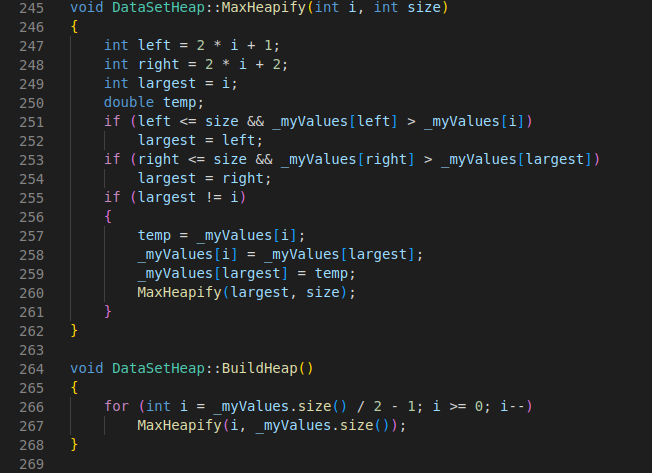
\includegraphics[width=.90\textwidth]{Heapify.png} % scale 75%
        \caption{Heapify}
\end{figure}
Max-heap data structure is used for this homework. It is a recursive function. Heap is builded just before "print" command. Building heap is the trigger function to construct the heap. Complexity of this algorithm is O(nlogn). Psuedo code can be seen as following:
\newpage
\begin{algorithm}[H]
	\caption{MAX-HEAPIFY}
	\label{algo:dfs}
	\begin{algorithmic}
	\State $l \gets LEFT(i)$
    \State $r \gets RIGHT(i)$
    \State $largest \gets i$
    \If{$l \leq heapsize[Vect]$ and $Vect[l] \geq A[i]$} 
		\State $largest \gets l$
    \EndIf
    \If{$r \leq heapsize[Vect]$ and $Vect[r] \geq Vect[largest]$} 
		\State $largest \gets r$
	\EndIf
    \If{$largest \neq i$} 
		\State swap Vect[i] and Vect[largest]
        \State \Call{max-heapify}{$largest$ , $Vect$}
	\EndIf
	\end{algorithmic}
\end{algorithm}

\begin{algorithm}[H]
	\caption{BUILD HEAP}
	\label{algo:dfs}
	\begin{algorithmic}
    \State $i \gets heapsize[Vect] / 2 -1$
    \For{$i > $0}\
    \State $i \gets i-1$
        \State \Call{max-heapify}{$largest$, $Vect$}
    \EndFor
	\end{algorithmic}
\end{algorithm}
\newpage
\subsection{Sorting}
\begin{figure}[H]
	\centering
	\label{fig:sort}
	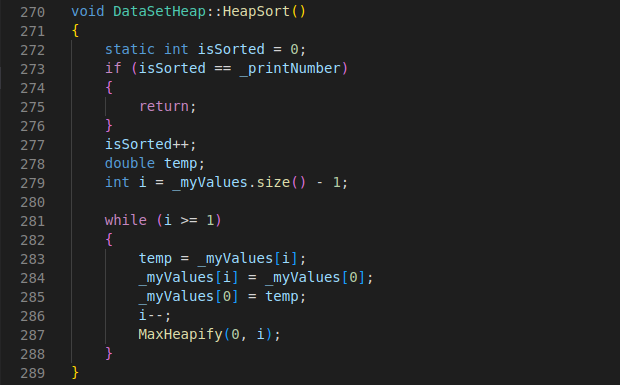
\includegraphics[width=.90\textwidth]{Heap Sort.png} % scale 75%
        \caption{Sorting}
\end{figure}
For sorting purposes, heap sort is used. First part of the code is for checking whether the heap is sorted or not.
Complexity is O(nlogn)
Sorting algoritm is called in these three case, during execution of code: 
\begin{itemize}
	\item First Quantile
	\item Median
	\item First Quantile
\end{itemize}
Rest of the algorithm can be seen as psuedo code:

\begin{algorithm}[H]
	\caption{HEAPSORT}
	\label{algo:dfs}
	\begin{algorithmic}
	\For{$i \gets heapsize[Vect]$ downto 1}
        \State swap Vect[0] and Vect[i]
		\State $heapsize[Vect] \gets heapsize[Vect]-1$
		\State\Call{max-heapify}{$0$ , $Vect$}
	\EndFor
	\end{algorithmic}
\end{algorithm}
\newpage
\subsection{Running Times}
This table shows the average runtimes for any cases. Each case tested 10 times at least.
\begin{table}[H]
	\label{table:runningtimes}
	\caption{Table of Running Times}
	\centering
	\begin{tabular}{| r | l |}
 \hline
input 1.txt  & 0.001 seconds \\
\hline
input firstq10.txt & 0.001 seconds \\
\hline
input firstq100.txt & 0.002 seconds \\
\hline
input firstq1000.txt & 0.022 seconds\\
\hline
input firstq10000.txt & 2.1 seconds\\
\hline
input firstq100000.txt & 3m58.879 seconds\\
\hline
input max10.txt & 0.001 seconds\\
\hline
input max100.txt & 0.004 seconds\\
\hline
input max1000.txt & 0.005 seconds\\
\hline
input max10000.txt & 0.09 seconds\\
\hline
input max100000.txt & 6.653 seconds\\
\hline
input mean10.txt & 0.001 seconds\\
\hline
input mean100.txt & 0.001 seconds\\
\hline
input mean1000.txt & 0.02 seconds\\
\hline
input mean10000.txt & 0.085 seconds\\
\hline
input mean100000.txt & 6.985 seconds\\
\hline
input median10.txt & 0.001 seconds\\
\hline
input median100.txt & 0.002 mseconds\\
\hline
input median1000.txt & 0.024 seconds\\
\hline
input median10000.txt & 2.166 seconds\\
\hline
input median100000.txt & 3m59.985 seconds\\
\hline
input min10.txt & 0.001 seconds\\
\hline
input min100.txt & 0.003 seconds\\
\hline
input min1000.txt & 0.005 seconds\\
\hline
input min10000.txt& 0.1 seconds \\
\hline
input min100000.txt& 6.235 seconds \\
\hline
input std10.txt& 0.002 seconds\\
 \hline
input std100.txt& 0.004 seconds\\
\hline
input std1000.txt& 0.012 seconds\\
\hline
input std10000.txt& 0.354 seconds\\
\hline
input std100000.txt& 34.109 seconds\\
\hline
input thirdq10.txt & 0.002 seconds \\
\hline
input thirdq100.txt & 0.004 seconds \\
\hline
input thirdq1000.txt & 0.029 seconds\\
\hline
input thirdq10000.txt & 2.457 seconds\\
\hline
input thirdq100000.txt & 4m04.164 seconds\\
\hline
\end{tabular}
\end{table}

\newpage
\subsection{Graphs}
\begin{figure}[H]
	\centering
	\caption{Graph}
	\label{fig:gta}
	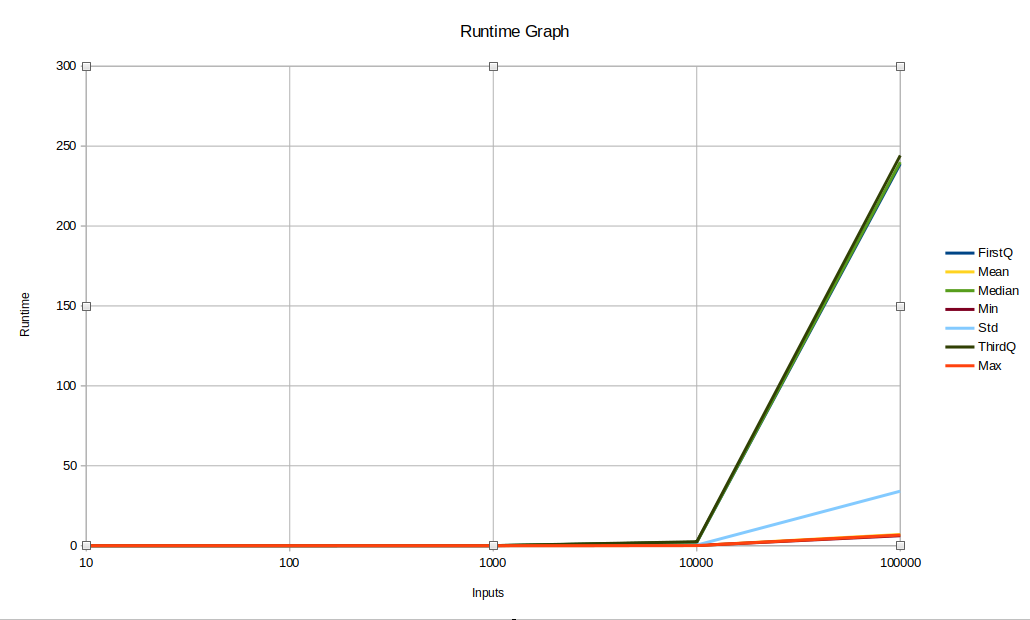
\includegraphics[width=.90\textwidth]{Graph.png} % scale 75%
\end{figure}
\newpage

\end{document}
